\documentclass[12pt]{article}
\usepackage[top=1cm, bottom=2cm, left=2cm, right=2cm]{geometry} 
\usepackage{hyperref}
\usepackage[style=authoryear, uniquename=false, backend=biber]{biblatex}
\usepackage{amsmath} %maths
\usepackage{graphicx}
\usepackage{import}
\usepackage{xspace}
\usepackage{perpage}
%
\renewcommand*{\thefootnote}{\fnsymbol{footnote}}
\MakePerPage{footnote}

\renewcommand{\c}{\textit{c.}\xspace}
\newcommand{\eg}{\textit{e.g.}\xspace}
\newcommand{\etc}{\textit{etc.}\xspace}
\newcommand{\ie}{\textit{i.e.}\xspace}
\renewcommand{\th}{\ensuremath{^{\mbox{\tiny th}}}\xspace}
\newcommand{\Nb}{\textit{N.b.}\xspace}
\newcommand{\nb}{\textit{n.b.}\xspace}
\newcommand{\ib}{{\boldsymbol i}}
\newcommand{\Xb}{{\boldsymbol X}}
\newcommand{\xb}{{\boldsymbol x}}

\newcommand{\Flat}{{\cal F}}
\newcommand{\screen}{{\cal I}}
\newcommand{\additive}{{\cal A}}
\newcommand{\qe}{{\cal S}}
%
\newcommand{\TBD}{\textit{T.B.D.}\xspace}
\newcommand{\XXX}[1]{\textbf{XXX #1}\xspace}

\bibliography{biblio,LSSTbiblio}

\begin{document}
\title{LSST's Plans for Calibrated Photometry}
\author{Robert Lupton, Mario Juri\'c, and Christopher Stubbs}
%\date{1996-03-06}
\maketitle
\tableofcontents

\section{Introduction}

In addition to photometry LSST needs to worry about calibrating astrometry and the PSF, but these
topics are not covered here.

In the notation defined in
``Level 2 Photometric Calibration for the LSST Survey'' \cite{LSE-180}.
the number of detected counts (\ie DN) $C_{raw, b}$ from an astronomical source with flux
$F_\nu$ in time $\Delta t$ in band $b$ is
$$
C_{raw, b} = \frac{\pi D^2 \Delta t}{4 g h} \int_0^\infty F_\nu(\lambda)
                                                   S^{atm}(\lambda) S_b^{sys}(\lambda) \,d\lambda/\lambda
$$
where $D$ is the telescope's effective diameter, $g$ the gain (photoelectrons per DN),
and $h$ Planck's constant.  The term `detected' is taken to mean those photons which are measured
as part of the PSF, as opposed to those spread out over the focal plane by scattering and ghosting.

We are interested in $S^{atm}$ and $S_b^{sys}$, the probabilities of a photon passing through 
the atmosphere and telescope/camera (including the mirrors, filter, and lenses) and being detected.  We shall
also need $S_{b, std}$, which we shall choose to be close to an average $S^{atm} S_b^{sys}$, probably
at an airmass of \c $1.2$.

Our task is, of course, to estimate $C_{std, b} \equiv \int_0^\infty F_\nu S_{b, std} \,d\lambda/\lambda$
given $C_{raw, b}$; doing this correctly requires knowledge of the object's SED.

Measuring $C_{std, b}$ splits into a number of separate operations, and we need to estimate:
\begin{itemize}
\item
  the detector sensitivity $S_b^{sys}(\lambda, \xb)$, including

  \begin{itemize}
  \item
    the atmospheric transmissivity $S^{atm}(\lambda)$
  \item
    the telescope (including optics and filters)
  \item
    the detector efficiencies
  \end{itemize}
  \item
  the object's SED
\item
  the background level and $C_{raw, b}$
\end{itemize}

\subsection{Absolute Photometry}

This document is written assuming that we can generate absolute photometry tied to NIST-certified
photo-diodes.  We accept that this is a radical and unproven approach, and in reality we will need externally
defined standards in order to either establish or validate our photometry.

One obvious possibility is dA white dwarfs, whose atmospheres (and circumstellar dust)
are thought to be understood at the 1-3\% level.

Another possibility that is at least amusing is to use SNe Ia's at a redshift where the cosmology is reliably
measured using BAOs ($a \approx 0.7$?); we would then use SNe Ia's at lower redshift to fill out the Hubble
diagram.

We defer a careful discussion of this issue to a later revision of this document.

\section{The instrumental sensitivity \texorpdfstring{$S_b^{sys}(\lambda, \xb)$}{Sb}}
\label{secInstrumental}

Measuring $S_b^{sys}(\lambda, \xb)$ requires us to measure the variation with $\xb$ (the flatfield)
and with $\lambda$ (the effective filter bandpass);  these two effects are not really separable.  We
must also ask what we mean by `effective filter bandpass':

A number of data sets are available to measure the \textit{in situ} sensitivity:
\begin{itemize}
  \item Broad-band dome flats
  \item ``Monochromatic'' (\c 1nm bandwidth) flats, calibrated with NIST photodiodes observing the calibration screen.
  \item Dithered star fields
  \item A set of spots from the collimated projector (see Appendix \ref{appProjector}).
\end{itemize}

Let $\screen(\lambda, \xb)$ be the illumination of the focal plane due to the illuminated flatfield screen
in the absence of telescope and filter effects;
we know the wavelength dependence of the screen illumination from the NIST diode data.

You might hope that $\screen$ would be a function only of $\lambda$ and the flatfield image $\Flat_b(\lambda,
\ib)$ would simply be to $\screen(\lambda)\,S_b^{sys}$; unfortunately your hopes are unfounded.

If the flatfield screen were at infinity, there was no vignetting, and the screen were perfectly Lambertian,
then non-uniform illumination of the dome screen would have no effect on the uniformity of $\screen$; in
reality these conditions are not all met and the illumination becomes $\screen_0 + i(\lambda, \ib)$.

$\Flat_b$ also includes
scattered light and ghosting (the latter a strong function of wavelength due to the details of the filter
$b$'s transmission function) so we must split $\Flat_b$ into multiplicative and additive parts:
$$
\Flat_b(\lambda, \ib) \equiv I(\lambda) \left(
                                              1 + i(\lambda, \ib) + \additive_b(\lambda, \ib)
                                        \right) \qe_b(\lambda, \ib)
$$
(assuming that the dome is light-tight and contains no glowing LEDs, in other words that $\Flat$ is
proportional to the illumination level).  We wrote $\qe_b$ not $S_b^{sys}$ because there are multiplicative
effects (\eg pixel size variations) other than quantum efficiency that enter into $\Flat_b$, and which
are included in $\qe_b$.

We expect the $\additive_b$ term to be a strong function of wavelength as reflections off the filter
are a significant contribution to the ghosts\footnote{
  if the filter transmission is $T(\lambda)$, the intensity that is reflected once and transmitted once
  is of course $T(1-T)$ and reaches 25\% at the 50\% point at the edge of the bandpass.
  }

We propose an approach to disentangling these effects in section \ref{secProjector}, and shall discuss how to
harness our knowledge of $\additive$ and $\qe$ in sections \ref{secFlatFielding} and \ref{secMeasuring}.

\subsection{Multiplicative Effects}

Structures seen in $\qe_b$ can come from either QE variations in the system (\eg dust on the filter or surface
annealing modulating the detector's sensitivity) and vignetting\footnote{
  The effects of vignetting and QE variation cannot be separated if we're considering light from the
  entire pupil as both lead to
lost photons; in the former case because they never reach the focal plane and in the latter because
the photon isn't absorbed by the detector.  This degeneracy is broken when we consider the collimated projector
in section \ref{secProjector}}, or changes in the effective size of the
pixels:
\begin{align*}
\qe_b(\lambda, \ib) =& \qe_b^{filt}(\lambda, \ib) \times \qe^{tel}(\lambda, \ib) \times \qe^{vig}(\lambda, \ib)
\times \qe^{qe}(\lambda, \ib) \times \qe^{geom}(\lambda, \ib)\\
\intertext{
  We may further split the `geom' part into optical distortion and CCD effects such as
  ``tree-rings'' or mask step errors:
  }
=&                     \qe_b^{filt}(\lambda, \ib) \times
                       \qe^{tel}(\lambda, \ib) \times
                       \qe^{vig}(\lambda, \ib) \times
                       \qe^{qe}(\lambda, \ib) \times
                       \qe^{optics}(\lambda, \ib) \times
                       \qe^{ccd}(\lambda, \ib)
\end{align*}
The last three terms are only a weak (or very weak) function of wavelength; they can vary due to chromatic
optical distortions and \eg variations in the importance of detector effects with conversion depth.

For measures of surface brightness QE/vignetting and geometrical effects are equivalent, but for measurements of objects'
fluxes we must be careful to separate them; treating larger pixels as more sensitive can give incorrect
results.%
\footnote{Flux is conserved, so if we are making a measurement of flux ignoring pixel size
  variation gives the correct result for all pixels which are given the same weight (\eg pixels entirely included in the aperture)}

The camera team will provide enough information to determine $\qe^{ccd}$; the details are \TBD.  The
$\qe^{optics}$ part will initially come from the optical design, but in production will come from the
astrometric solution which will determine it with exquisite precision.  We only need to know $\qe^{vig}$ in
order to make an \textit{ab initio} model of the system, and to estimate the importance of non-uniform
illumination of the flatfield screen.\footnote{
  We also theoretically need it to measure the filter profiles using a widget such as that
  mentioned in a footnote in section \ref{secFilterProfiles}.
  }

\subsection{Using Star Flats}
\label{secStarFlats}

The classical solution to this problem is to take the dome flat at face value as a measure of quantum
efficiency, then take a number of exposures of a star field at a set of boresight offsets, flatfielding using
our dome-based flat fields.  If we make the reasonable assumption that most of the stars are not variables, we
may setup and solve a system of linear equations for a model of a reasonably slowly varying correction to the
domeflat --- the illumination correction --- and also the brightnesses of all the stars (here just a set of
nuisance parameters); the combination of this illumination correction and the domeflat is $S_b^{sys}(\lambda, \ib)$.

Because we are interested in the effects of objects' SED on their photometry we would have to generalise this
to make use of the colours of the stars.  It seems possible that this would enable us to measure the
wavelength dependence of the spatial structure of the illumination correction well enough to produce reliable
colours for stars and normal galaxies, but it's improbable that the diversity of star colours is large enough
to measure it well enough to handle an arbitrary SED.

\subsection{Using the Collimated Projector}
\label{secProjector}

As discussed in Appendix \ref{appProjector}, we will be able to project a mask with a set of holes onto the
focal plane.  Each hole produces a \c 50pixel spot\footnote{Available projectors are close to diffraction
  limited, and with a 30cm diameter we should be able to produce images as small as 0.7'' FWHM at $1\mu m$.
  }
  and a series of ghosts;  the density of holes in the
mask will be chosen to allow us to separate the primary spots from the ghosts, possibly using an optical model
of the system.  In the discussion of $\Flat$ above we implicitly defined the system throughput to be the
fraction of the incident light that is detected in the primary spot, with the ghosts creating $\additive$.

Because our projector only illuminates a small portion of the primary we need to extend
our notation (and writing $\qe^{tel, vig} \equiv \qe^{tel} \qe^{vig}$):
$$
\Flat_b(\lambda, \ib) \equiv I\, \qe^{qe, optics, ccd} \int_{pupil} \left(
                                                                1 + i + \additive_b
                                              \right) \qe_b^{filt} \qe^{tel, vig}\, d\Xb
$$
Note that an integral over the pupil is automatically an integral over photon arrival directions.  We
are assuming that \eg the effective size of the pixel isn't a function of the incident angle of the photon,
which seems likely to be very nearly true (although this assumption isn't fundamental).

We may write the total flux in the primary image of the $\ell^{th}$ spot imaged through the $b$ filter in a narrow
range around wavelength $\lambda$ at the point $\xb_i$ as
$$
P_b^\ell(\lambda, \xb_i, \Xb) = a^\ell I(\lambda)\, (1 + i(\lambda)) \qe_b^{filt}(\lambda)
 \qe^{tel, qe, vig, optics, ccd}(\lambda)
$$
and, if we take a series of exposures that collectively illuminate the entire primary (and dropping
the explicit $\lambda$ for readability) we may evaluate
$$
P_b^\ell(\xb_i) = a^\ell I\, \qe^{qe, optics, ccd}
                   \int_{pupil} (1 + i) \qe_b^{filt} \qe^{tel, vig}\,d\Xb
$$
At this point we know the relative spectral response at a set of points in the focal plane.                   

If we now move these spots around the LSST focal plane, taking data at only a single position in the pupil and
wavelength, we may solve for the relative sensitivities between the spots $\{\ell\}$ in a manor exactly
equivalent to star-flat approach of section \ref{secStarFlats}.\footnote{ This rasterisation is a little tricky.  If
  we simply tilt the projector to move the spots they will illuminate a different part of the primary; if also
  move the projector we can arrange that the footprint on one of the optical elements (primary, secondary,
  filter, ...) remains fixed.  As an alternative we can move the mask relative to the projector's optic axis
  and adjust the projector to keep the spots fixed; we can then solve for the variation of brightness around
  the projector's focal plane.  If this is stable we can then translate the mask when determining the
  individual holes' throughputs.  In reality we would do both.  }
We would repeat this analysis at a (sparse) set of wavelengths to check for chromatic effects in the hole's
throughputs due to \eg diffractive effects

Once we know the $a^\ell$'s, we scale all the spot intensities to a common scale,
$$
P_b^\ell(\xb_i) = I\, \qe^{qe, optics, ccd} \int_{pupil} (1 + i) \qe_b^{filt} \qe^{tel, vig}\,d\Xb
$$
and
$$
\Flat_b(\lambda, \xb_i) = P_b^\ell(\xb_i) + I\, \qe^{qe, optics, ccd}
                              \int_{pupil} \additive_b \qe_b^{filt} \qe^{tel, vig}\, d\Xb
$$
If, as would be expected, the first term varies only slowly over a chip, then rastering the spots to
illuminate some number \TBD of positions on each chip allows us to $P_b^\ell(\ib)$, \ie at every pixel.
Unfortunately we still don't know how to find the pixel-to-pixel variability.  If there is a clear
separation between the spatial scales probed by $P$ and $\Flat$ (\ie and $\additive$) we can combine
the two estimates to generate a flatfield uncontaminated by scattered light and ghosting.

For many cameras the spatial structure of $\additive$ has sharp features.  Furthermore, the operations
described above are expensive (see Table \ref{tab:NExposure}), and we have to repeat for every \c 1nm step
in wavelength.  If we know
the filter bandpasses $\qe_b^{filt}(\ib)$ at every point in the focal plane (see section
\ref{secFilterProfiles}) we may use a slightly different approach.

If we take both domeflat and collimated projector data without a filter in the beam\footnote{
  The projector beam is so slow that the
  image quality should not be significantly degraded} we may repeat
the above analysis without the $\qe_b^{filt}$.  This has two advantages: there are
no strongly chromatic elements so we can use larger steps in wavelength;  and the $\additive$
image should be much weaker (as much of it comes from the filter edges).  Having \XXX{achieved a
separation of scales}, we have measured
$\qe^{qe, optics, ccd, tel, vig}(\lambda, \ib)$ and knowing $\qe_b^{filt}(\lambda, \ib)$ we have
measured our desired sensitivity with only one remaining contaminant: the non-uniform illumination
resulting from an imperfect flatfield screen, $i$ (see next section).

\subsubsection{Characterising the Ghosts}

We have worked hard to avoid contaminating our $\qe$ estimates with ghosts and scattered light, but
we can now carry out a consistency check.  In addition to the $P_b^\ell(\lambda)$ we can \XXX{probably}
measure the ghosts, $G_b^\ell(\lambda)$.  By interpolating and then summing over the focal plane
we have an estimate of $\additive_b$;  it will be interesting to see how well this works.

\subsection{Non-uniform Dome Flat Illumination, \texorpdfstring{$i$}{i}}

Because the screen isn't at infinity and because of vignetting, surface brightness variation over
the flat field screen leads to spatial structure in the focal plane: $i \ne 0$.

We may get a handle on this surface brightness by employing a pinhole camera in place of a
filter.
\XXX{Chris Stubbs worries that the angular distribution of light imaged by this camera
  is very different from the domeflat illumination; \c $f/1$ as opposed to only within 1.75$^\circ$ of normal.
  which would require us to know the screen's BDRF to make appropriate corrections.  I don't see this,
  as the pinhole is in the same beam}
Alternatively, we expect the effects of $i$ to be have only weak spatial and spectral variability.  If this
is the case, we can use dithered star fields to make a correction.

\subsection{Measuring the Filter Profiles}
\label{secFilterProfiles}

We may have lab measurements of the filter profiles at a dense grid of points over the filters.\footnote{
  For example by scanning an beam with the appropriate range of f-ratios to simulate the LSST beam
  across the filter and collecting the transmitted light into a spectrophotometer}

Alternatively the unfiltered data also allows us to measure (or monitor) the filter bandpasses.  As mentioned
above, scanning a spot in wavelength measures the sensitivity of a point in the focal plane, so the ratio of
the sensitivity measured with and without the filter is the filter bandpass:
\begin{align*}
  \frac{P_b^\ell}{P_{clear}^\ell} =& \frac{\int_{pupil} (1 + i) \qe_b^{filt} \qe^{tel, vig}\, d\Xb}
                                          {\int_{pupil} (1 + i) \qe_{clear}^{filt} \qe^{tel, vig}\, d\Xb}\\
\end{align*}
(again assuming that $\qe^{qe, optics, ccd}$ are not dependent on $\lambda$).  If $i$ is well behaved (\eg
Lambertian) this is exactly what we want, with the correct average over the rays traversing the filter.

\subsubsection{Fringing}

There is one extra wrinkle.  CCDs behave like Fabry-Perot cavities, and this modulates the throughput. Because
the spatial variability comes from thickness variations in the devices it can have fine scale structure, and
the correct way to measure this is with a white-light flat-field exposure taken at \c 1nm spacings.  We
include an estimate of how long it would take to acquire this data in Section \ref{sec:CalibrationExposures},
but it is not obvious if this is really necessary.

Fringing in the LSST chips is expected to be small as not only are the devices thick, so little light is
returned from the bottom of the device to interfere, but also the very fast beam washes out the
effect. Preliminary estimates (\cite{document-8590}) suggest that fringing will not be important for
LSST, but we believe that it would be premature to ignore its effects.  Note that fringing is important
even in the absence of strong emission lines;  lines produce clear artifacts in the sky brightness, but
interference modulates the sensitivity even for continuum sources.

\section{The atmospheric transmissivity \texorpdfstring{$S^{atm}(\lambda)$}{Satm}}

The current baseline plan is to use a 1.2m telescope with $R \sim $ 300 --- 400 to take spectra of standard
stars with a cadence of \c 5 minutes (3 minutes to integrate; 2 minutes to slew and acquire).  The expected
S/N at 12$^{th}$ magnitude is 500/resolution element (300 in u and y).

There will also be two units to measure water vapour;  a all-sky monitor using GPS satellites
and a bore-sight mounted radiometer to measure the vertical profile.

The baseline proposal is to use these spectra to find the atmospheric absorption along the line of sight to
standard stars (\nb with a inter-visit time of 5 minutes there will be \c one exposure per 10 LSST visits).
We will then decompose the atmospheric transmission into a set of basis functions and use these to interpolate
in space and time to find $S^{atm}$ at any position in the focal plane.

The task of reducing these data has two phases:
\begin{itemize}
  \item Generate calibration products sufficient to extract accurate spectrophotometry from 2-d spectra
    \XXX{What these are needs to be sorted out; do we need a monochromater in addition to quartz and arc
      lamps?}

  \item Define $n$ components which describe $S^{atm}$.  These could come either from
    from MODTRAN (with modified aerosol absorption properties estimated from the data) or
    a PCA-like decomposition of all the data we've already taken.
    This latter choice is not able to detect a
    constant (but chromatic) component -- we're only sensitive to the variation in the atmospheric properties.
    This decomposition must be able to interpolate in airmass over
    a limited range (the scale is between half the LSST focal plane and \c 3 times larger if the auxiliary
    telescope cadence is 10 times slower than the main telescope).

  \item Acquire ``ground truth'' spectro-photometric spectra for all stars that will be observed by the
    auxiliary telescope.  \eg Using the auxiliary telescope, booststrap from dA white dwarfs with
    known SEDs \XXX{Are WD SEDs really known well enough?  1-2\%?}.  \nb  Again, we could bootstrap
    these SEDs from the data given enough observations, subject to an overall constant chromatic scaling;
    this seems much scarier than determining the atmospheric components from the data.
\end{itemize}

Then, for each exposure,
\begin{itemize}
  \item Remove the instrumental signature from the 2-d data.
  \item Extract a wavelength and intensity calibrated 1-d spectrum, presumably using a 1-d `optimal'
    extraction algorithm.
  \item Given the known spectrum of the object and the extracted spectrum, fit the parameters describing the
    atmosphere.
\end{itemize}
\nb we would probably really combine these two steps and directly fit for the
atmospheric parameters given the post-ISR 2-d data

\XXX{It is a non-trivial task `Extract a wavelength and intensity calibrated 1-d spectrum'}

\subsection{Required S/N}

The base-line plan expects a S/N of 300 --- 500 per resolution element for a \XXX{180s} integration on a
12$^{th}$ magnitude star, with $R \sim 400$ (a total S/N of \c 6000 --- 10000).  This will be used to
determine \c 6 parameters describing the atmospheric transmission.

Apart from the overall cloud extinction (a serious problem with which this telescope does not help), these
numbers will result in corrections of at most 3\%, so we need to know them in turn to 3\% to achieve 1mmag
photometry, \ie an S/N of \c 30; with 6 parameters we need a total S/N of \c 200 which can be achieved in \c
7s for a 12$^{th}$ magnitude object.  Alternatively, given a 180s exposure we can use stars as faint as 15.5.

The overhead between exposures is currently thought to be \XXX{120s}, so there's no point going significantly
below a 60s exposure unless we can build a more agile auxiliary telescope.

\subsection{Stellar Photometry}
\label{secStellarPhotometry}

\begin{figure}
\begin{center}
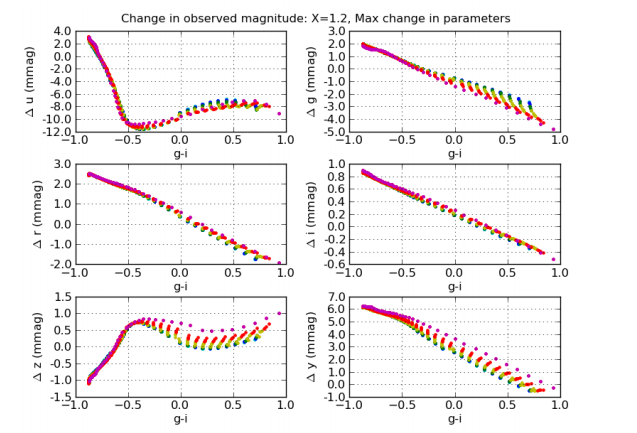
\includegraphics[width=14cm]{maxAtmosphereDeltas}
\end{center}
\caption{
  \label{figMaxAtmosphereDeltas}
  The change in the observed magnitude of stars in the temperature range 5000---35000K as the properties
  of the atmosphere are changed between two extreme models, keeping the airmass fixed at 1.2.  The different
  coloured points correspond to a range of metallicity and gravity.
  }
\end{figure}

To determine the optimal use of auxiliary data we need to see what can be learned directly from the
photometry and what information must come from elsewhere.

We will have many-colour photometry (\textit{ugrizy}) of \XXX{many, many} stars in each visit.  We know from
simulations of Kurucz models that as the properties of the atmosphere are varied there are several percent
level changes in fluxes, with percent-level scatter at a given $g - i$ colour (See figure
\ref{figMaxAtmosphereDeltas}).  It is not yet clear how much of this scatter can be regressed out using all
five available colours (see also section \ref{secSED}). If the
conditions are not photometric this is not an insuperable problem as the positions of red and blue
stars do not correlate with the regions of dense cloud --- but it does make it harder.  If the structure
of the extinction is sufficiently complex we will not be able to reach SRD precision independent of
our ability to correct for the subtle effects of the atmosphere.

Even if the scatter can be removed to SRD precision (see appendix \ref{appSRD}), it is not clear how well
we will be able to characterize $S^{atm}$ across the filter $b$.  In reality the solution should use all
available information (\eg satellite-based ozone; atmospheric pressure; water-vapour).

\XXX{We need to do a study on way of characterising the atmosphere. Probably the $i$-band is the most
interesting as it is subject to effects from aerosols (two parameters), water vapour (one), and \XXX{Rayleigh scattering} (one).}

\subsection{Spatial Structure of the Atmosphere}

Even if the photometry is unable to constrain $S^{atm}$ well enough to satisfy the SRD requirements, it seems
very likely that we will be able to say something interesting.  Once we have implemented an initial version of
the photometric analysis we will be able to analyse wide-field camera data to explore the structure functions.
Obvious candidates are SDSS stripe82, DECam, and HSC.  These cameras have obvious tradeoffs in data
availability, available integration times, maximum scale probed and object density (and hence spatial
resolution).

\section{Flatfields}
\label{secFlatFielding}

Section \ref{secInstrumental} discusses analysing the response to the flatfield screen,
$(1 + i + \additive_b) \qe_b^{filt} \qe^{tel} \qe^{qe} \qe^{optics} \qe^{ccd}$.
Before we can create a flatfield image for band $b$ we need to:
\begin{itemize}
\item Decide what to do about $i(\lambda, \ib)$
\item Decide what to do about $\additive_b(\lambda, \ib)$
\item Decide what to do about $\qe^{optics}(\lambda, \ib)$
\item Decide what to do about $\qe^{ccd}(\lambda, \ib)$
\item Choose an SED
\end{itemize}

Correcting for $i$ is always desireable and we shall assume that it's been accomplished.\footnote{A better
  solution would be to design a flatfield screen which delivers $i \equiv 1$} It might seem obvious that the
flatfield should exclude $\additive$ and correct for $\qe^{optics} \qe^{ccd}$, resulting in a map of the
detector's true QE.  However, this is probably not a good idea as it
\begin{itemize}
\item leads to a complex background image
\item does not remove the need for sufficiently scrupulous algorithms to require access to the per-pixel
  geometrical information.
\end{itemize}

Once the data is warped to \eg a tangent plane these geometrical effects on QE are removed (the resampling
kernels include the determinant of the transformation's Jacobian).\footnote{ The inevitable distortion of the
  new projection will of course lead to a new $\qe^{optics}_b$.  } It would be possible to remove the effects
of the dimensions of individual pixels at the same time, but we shall choose to forgo this option; see the
discussion of background estimation in section \ref{secMeasuring}.

Removing $\additive_b$ from the flatfield also complicates the background, adding the scattered light and ghosting
back into the data.  As background estimation is already a challenging task (even with background matching),
this seems undesirable.

We therefore propose that the flatfields be calculated as follows:
\begin{itemize}
  \item Use the sky's SED modified by $\qe_b^{filt}$. We could use different sky models for different phases
    of the moon (or solar cycle), or measure the sky emission directly (possibly using the calibration
    telescope). We will need to at least allow for the phase of the Moon.

  \item Do not correct for $\additive_b$ (resulting in an incorrect estimate of the sensitivity).

  \item Correct for $\qe^{tel} \qe^{qe}$

  \item Correct for $\qe^{optics}$

  \item Do not correct for $\qe^{ccd}$
\end{itemize}
This is the flatfield that best flattens the sky once warped onto a tangent plane,
at the cost of photometric errors.
We will need to include fringe frames made from medianed sky exposures in the sky model, but the 
dimensionality of the required fringe set is not yet clear. \XXX{Expand at some point}

We will further discuss the consequences of this choice in section \ref{secMeasuring}.

\subsection{Flatfields for Level 1}

This description is appropriate for level 2 processing, but level 1 is different and we must ensure that the
choices made during flatfield generation matches the adopted processing flow.  It may turn out that we need
different level 1 and level 2 flats.

\section{The object's SED}
\label{secSED}

Let us remember that we don't actually need to know the SED; we need merely to know enough about it to allow
us to make sufficiently accurate corrections from $C_{raw, b}$ to $C_{std, b}$.

We don't know our objects' SEDs, but we do know their multi-band fluxes $\{C_{std,b}\}$\footnote{
  the distinction between \eg $std$ and $nat$ fluxes doesn't really matter here,  but if necessary
  we could iterate the calibration procedure until we arrive at $C_{std, b}$.
  }
and other parameters
$\theta$ (\eg morphological information).  There is a probability distribution
$p({\rm SED}|\{C_{std, b}\}, \theta)$ which
may be compact, essentially reducing to a single reasonably well-defined SED, or may reflect the intrinsic
range of SEDs of objects with those properties.\footnote{
  In reality galaxies display colour gradients; we'll return to this in section \ref{secMeasuring}.
}
The parameters $\theta$ may include morphology (adopting different SEDs for stars and galaxies), or
Galactic $(l, b)$ if we wish to take Galactic reddening into account.

If we restrict our attention to stars, the colours probably determine the SED reasonably well (see
section \ref{secStellarPhotometry}).  Studies of galaxies' photometric redshifts tell us that their SED is
often, but not always, reasonably well defined by the colours; QSOs show significant degeneracies, mostly
at redshifts below \c 2.5.

There is nothing we can do about this degeneracy, which means that we cannot hope to correctly estimate
$C_{std, b}$ for a subset of objects which we detect.  However, we will need to define a deterministic mapping
from colour to $\mbox{SED}(\{C_b\}, \theta)$ which will allow a consumer of the data to make their own
correction (see section \ref{secMeasuring}).

If an object appears \textit{ex nihilo} we know nothing about its SED, so we shall have to adopt
some spectrum (\eg a flat-spectrum source) and increase the error estimate accordingly.  This is unlikely
to be important as the SED-based corrections are small.

\section{Measuring the background level and \texorpdfstring{$C_{std, b}$}{Cstd}}
\label{secMeasuring}

\subsection{Background Subtraction}

We plan to background match multiple exposures of a patch of the sky in a given filter before sky subtraction,
generating a stacked image in a sky projection.

This results in two data products:
\begin{itemize}
\item The background image in the stacked image $B^{stack}$.
\item The differences $B^i$ between this background image and the input images.
\end{itemize}
Because we measure $B^{stack}$ in sky coordinates the geometrical distortion terms $\qe^{optics}$ in
the flatfield illumination are automatically removed,\footnote{They are replaced by $\qe^{projection}$,
  but this term is not dependent on the boresights of the visits.}
and when we warp $B^i$ back to the corresponding
calibrated raw frame and subtract it we arrive at an image with $\qe^{optics}$ fully accounted for.

If we had included $\qe^{ccd}$ in the flatfield we would have handled the background correctly if we also
included it in the warps to and from sky coordinates, but we would not be able to forget about it as it
continues to have effects on the astrometry and photometry.\footnote{ it would also have made the warp code
  more complex and probably slower as the individual area of each pixel would have to be handled explicitly.
}

Having removed the background we can reconsider the choices we took when we built our flatfields
(section \ref{secFlatFielding}).
\begin{itemize}
   \item We no longer have any motivation to use the sky's SED (as we have subtracted all the sky photons),
     but do not know what to use instead to get the correct fluxes for the object photons.
   \item We should now correct the sensitivity for the effect of $\additive_b$ as it no longer complicates
     the sky subtraction.
   \item We could decide to now correct for $\qe^{ccd}$.
\end{itemize}

\subsection{Measuring \texorpdfstring{$C_{std, b}$}{Cstd}}

All photometric measurements can be thought of fitting a model $M$; $I = a M$.  Let us take this
model to describe the image above the atmosphere, and to be in photons not Joules.
We know our object's $(\{C_b\}, \theta)$, so we know which SED we should adopt (section \ref{secSED}).

The signal that we measure after (incorrectly) flat fielding with a flat constructed using the sky's SED is
$$
I_j = a \int_{b} S_{obj}^{atm} \frac{\qe_{b, j, obj}^{filt} \qe_{j,obj}^{tel} \qe_{j,obj}^{qe}}
                                    {\qe_{b, j, sky}^{filt} \qe_{j,sky}^{tel} \qe_{j,sky}^{qe}}
            \qe_j^{ccd} M_j P_b(\lambda)\, d\lambda + \epsilon_j
    \equiv a w_j + \epsilon_j
$$
where $I_j$ is the intensity of the $j^{th}$ pixel and $\epsilon_j$ the noise.  I'll drop the explicit
integral over filter $b$'s bandpass $P_b$ so all sensitivities in this section should be taken to be
bandpass-averaged.

If we take the $\epsilon_j$ to be independent Gaussians $N(0, \sigma_j^2)$, the maximum likelihood estimate
for the amplitude $a$ is
$$
a = \frac{\sum_j w_j I_j/\sigma_j^2}{\sum_j w_j^2/\sigma_j^2}
$$
and the total number of DN $C$ is $C = a\sum_j w_j$
(this is an unbiased estimate even if the errors aren't Gaussian).
It is almost always best
to set $\sigma^2_j = 1$ to avoid systematic errors as a function of magnitude, and we shall do so
in this discussion.

Let us assume that the ratios  $\qe_{b, obj}^{filt}/\qe_{b, sky}^{filt}$ 
$\qe_{obj}^{tel}/\qe_{sky}^{tel}$ and $\qe_{obj}^{qe}/\qe_{sky}^{qe}$ are
constant for all the pixels in the object.  This isn't necessary, we can handle it the same way as we'll
handle $\qe_j^{ccd}$, but it is probably a good assumption and has some advantages.  In this case, we have
\begin{align*}
  a =& \frac{1}{S_{obj}^{atm}} \frac{\qe_{b, sky}^{filt} \qe_{sky}^{qe}}
                                    {\qe_{b, obj}^{filt} \qe_{obj}^{qe}}
                         \frac{\sum_j (\qe_j^{ccd} M_j) I_j}{\sum_j (\qe_j^{ccd} M_j)^2}\\
C =& a \sum_j \qe_j^{ccd} M_j\\
\intertext{and, correcting to a standard atmosphere, and writing $w = \qe_j^{ccd} M_j$}
C_{std} =& \frac{S_{obj,std}^{atm}}{S_{obj}^{atm}}
                  \frac{\qe_{b, sky}^{filt} \qe_{sky}^{qe}}
                       {\qe_{b, obj}^{filt} \qe_{obj}^{qe}}
                         \, \frac{\sum_j w_j I_j  \sum_j w_j}{\sum_j (w_j)^2} \\
\equiv& \frac{S_{obj,std}^{atm}}{S_{obj}^{atm}}
                  \frac{\qe_{b, sky}^{filt} \qe_{sky}^{qe}}
                       {\qe_{b, obj}^{filt} \qe_{obj}^{qe}}
                         \, C_{raw}
\end{align*}

\newcommand{\cSED}{c_{\scriptscriptstyle\rm SED}}

If we have $n$ exposures this generalises to
\begin{align*}
C_{std}  =& \sum_r
    \frac{S_{obj,std}^{atm}}{\qe_{obj}^{atm,r}}
    \frac{\qe_{b, sky}^{filt,r} \qe_{sky}^{qe,r}}
         {\qe_{b, obj}^{filt,r} \qe_{obj}^{qe,r}}
    \, C_{raw}^r\\
 \equiv& \sum_r \cSED^r C_{raw}^r
\end{align*}
I have kept the per-visit superscript $r$ in $\qe^{filt}$ to allow for spatial variation in the filter
properties, and in $\qe^{qe}$ to allow for different CCDs in the focal plane having different sensitivities.
If you think that the different platescale for object- and sky-coloured objects have a significant effect, you
may add the ratio $\qe_{sky}^{tel}/\qe_{obj}^{tel}$ but it seems unlikely that this will be necessary.

\XXX{Note that we can correct for a different SED without keeping the $C_{raw}^r$}

Note that the SED doesn't enter into the pixel-dependent part, $C_{raw}^r$, making it relatively simple to
adopt a different SED and recalculate $C_{std}$ if we know the $\cSED^r$.  We don't need to save $\cSED^r$
for every object as we only need the SED, and that is known given $(\{C_b\}, \theta)$.  This simplification
depends on our assumption about the constancy of  $\qe_{obj}^{tel}/\qe_{sky}^{tel}$ and
$\qe_{obj}^{qe}/\qe_{sky}^{qe}$ over the object.

\subsection{Colour Gradients}

Because we using a model-based approach to handle SED dependencies we can easily handle more complicated
problems; for example, if we are using a bulge/disk decomposition we are estimating the colours of each
component, and can handle their SEDs separately when fitting our model.

\appendix

\section{The Collimated Projector}
\label{appProjector}

A source of monochromatic light, driven by a light source equivalent to that used to illuminate the flatfield
screen, capable of projecting an image mask (\eg a set of spots) onto the focal plane.  If we consider a mask
with a single aperture the output is a parallel light with diameter equal to the diameter of the projector's
exit pupil.  This beam illuminates a small patch on the LSST's primary mirror, and is focused as a spot on the
focal plane.  For a 30cm aperture projector the area illuminated is \c 0.2\%; the beam diameter is \c 20\%
of the annular radius of M1.

By using diffraction limited optics and a 10cm projector we can generate a beam with a divergence of \c 1
arcsec, which is then imaged into a 1 arcsec spot by the LSST optics; a larger projector could generate
\c pixel-sized spots, allowing us to investigate PSF effects that were not resolved before the camera
is fully assembled.  When used for its primary photometric purpose we expect to generate \c 50-pixel
spots.

In reality we can generate a number of spots simultaneously by putting an image mask in the projector's focal
plane.  The projector's output beam then diverges at 3.5$^\circ$, illuminating an area with diameter \c 60cm;
each focused spot still only illuminates a patch the size of the exit pupil of course.  We may not assume that
each spot is equally bright; not only are the holes in the image mask not going to be all identical, but the
projector illumination is expected to vary slightly across the mask.

In addition to the direct image the projector will generate a series of ghosts, which form a set
of distorted images of the pupil.  Because the projector beam only illuminates a small portion of
the primary, the projector ghosts are proportionally smaller than the full-pupil ghosts.

\import{.}{calibrationExposures}

\section{Science Requirements Document (SRD)}
\label{appSRD}

The SRD specifications are:

\begin{description}
\item{Repeatability}\\
  the median value of the photometric scatter for each star (the rms of calibrated
  magnitude measurements around the mean calibrated magnitude) shall not exceed 5 millimags in gri, 7.5
  millimags in uzy. No more than 10\% of these objects should have a photometric scatter larger than 15 mmag
  in gri, 22.5 mmag in uzy. This requirement sets the level above which we can reliably detect intrinsic
  variability in a single source.
  
\item{Uniformity}\\
  the rms of the internal photometric zeropoint error (for each visit) shall not exceed 10
  millimags in grizy, 20 millimags in uzy. No more than 10\% of these sources can be more than 15 mmag in gri
  or 22.5 mmag in uzy from the mean internal zeropoint. This places a constraint on the stability of the
  photometric system across the sky as well as an upper limit on various systematic uncertainties, such as any
  correlation of photometric calibration with varying stellar populations (or colors). This makes the
  photometry of sources directly comparable over the entire sky, and when combined with the previous
  requirement, creates a stable photometric system across the sky and over time, in a single filter.

\item{Band-to-band photometric calibration}\\
  The absolute band-to-band zeropoint calibration for main sequence
  stars must be known with an rms accuracy of 5 millimags for any color not involving u band, 10 millimags for
  colors constructed with u band photometry. This requirement ties photometric measurements in different
  filters together, enabling precise measurement of colors, and allows LSST photometry to be compared with
  that from other optical telescopes, and with astrophysical models.

\item{Absolute photometric calibration}\\
  The LSST photometric system must transform to an external physical
  scale (\eg AB mags) with an rms accuracy of 10 millimags. This is essential for comparing with photometry
  from other wavelength regions, such as IR or UV.
\end{description}

\section{Glossary}

\begin{description}
  \item $\additive$\\
    The part of $\Flat$ that is due to scattered light and ghosting, \ie is not proportional
    to the effective quantum efficiency of the detector.      

  \item{BDRF}\\
    Bi-Directional Reflection Function; the reflectivity of a surface in \textit{this} direction
    in response to incident light from \textit{that} direction.

  \item{DN}\\
    Data Number; the value of a pixel as read from the detector (also called ADU)

  \item $\Flat$\\
    The image of the flatfield screen in the $b$ band (\ie the data resulting from illumination
    of the camera with $\screen$).

  \item{ISR}\\
    Instrumental Signature Removal (remove bias, flatfield, \etc)

  \item $\screen$\\
    The illumination of the focal plane due to the flatfield screen; the light intensity
    just above the front surface of the detectors in the absence of telescope and filter effects.

  \item $i$\\
    The pattern of non-uniform illumination of the focal plane in the absense of any telescope or camera
    effects except for the effects of vignetting (but corrected for the geometrical part of the
    vignetting --- that is, the fraction of the pupil visible from a point in the focal plane).

  \item{QE}\\
    Quantum Efficiency

  \item $P_b^\ell(\lambda, \xb_i, \Xb)$\\
    The total flux in the primary image of the $\ell^{th}$ Stubbs Spot imaged through the $b$ filter in a
    narrow range around wavelength $\lambda$ at the point $\xb_i$.
    
  \item $\qe$\\
    The effective quantum efficiency of a pixel.
    \begin{description}
    \item $\qe^{tel}(\lambda, \ib)$
      The probability of a photon incident on the pupil reaching the detector (neglecting vignetting
      and the filter)
    \item $\qe_b^{filt}(\lambda, \ib)$
      The probability that filter $b$ transmits a photon
    \item $\qe^{qe}(\lambda, \ib)$
      The probability of a photon incident on the detector being detected
    \item $\qe^{vig}(\lambda, \ib)$
      The probability that a photon incident on the pupil will not be vignetted
    \item $\qe^{optics}(\lambda, \ib)$
      The effective area of a pixel (in units of nominal pixels) allowing for distortions
    \item $\qe^{ccd}(\lambda, \ib)$
      The effective area of a pixel (in units of nominal pixels) allowing for physical changes
      in the size of the pixel (\eg `ragged gates').
    \end{description}

  \item $S^{atm}$\\
    The probability that a photon will pass through the atmosphere for a given visit.

  \item $S_b^{sys}$\\
    The probability that a photon will pass through the telescope and camera (with the $b$ filter)
    and be absorbed by the detector;  assumed to vary relatively slowly with time.

  \item $S_{b, std}$\\
    The probability that a photon incident on the atmosphere will be detected under `standard' conditions; all
    photometry is referred to this probability.

  \item{SED}\\
    Spectral Energy Distribution

  \item{S/N}\\
    Signal-to-noise ratio

  \item{SRD}\\
    Science Requirements Document

  \item{TBD}\\
    The meaning of this acronym is To Be Decided

  \item{$\xb$}\\
    Coordinates in the focal plane.  A function defined at a point is written $f(\xb_i)$,
    whereas a function defined at all pixels is written $f(\ib)$.

  \item{$\Xb$}\\
    Coordinates in the pupil.
\end{description}

%------------------------------------------------------------------------------

\printbibliography[heading=bibintoc]

\end{document}
